\documentclass{article}
\usepackage{amsmath}
\usepackage{listings}
\usepackage{amssymb}
\usepackage{color}
\usepackage{graphicx}
\parindent=19pt
\begin{document}
\title{Finite Element Method}
\author{Wei Zhang}
\large
\maketitle

\section{Exercise 10: Finite Element Algorithm by hand}
The nodes: $[0, \pi/2, \pi]$, the elements $[0, 1],[1, 2]$.
\begin{equation*}
\displaystyle\varphi_{0}=1-\frac{x}{\displaystyle \pi/2},     ( 0\leq x\leq\frac{\pi}{2})
\end{equation*}

\begin{equation*}
\displaystyle\varphi_{1}=
\begin{cases}
\displaystyle\frac{x}{\pi/2} & \text{ $\displaystyle0\leq x\leq\frac{\pi}{2}$}\\
\displaystyle 1-\frac{x-\pi/2}{\pi/2} & \text{ $\displaystyle\frac{\pi}{2}< x\leq\ \pi$}
\end{cases}
\end{equation*}

\begin{equation*}
\displaystyle\varphi_{2}=\frac{x-\pi/2}{\pi/2},     ( \frac{\pi}{2}\leq x\leq\pi)
\end{equation*}


\begin{equation}
\hat{u}=
\begin{cases}
c_{0}\varphi_{0}+c_{1}\varphi_{1}& \text{$\displaystyle 0 \leq x \leq \frac{\pi}{2}$}\\
c_{1}\varphi_{1}+c_{2}\varphi_{2}& \text{$\displaystyle \frac{\pi}{2}< x \leq \pi$}

\end{cases}
\end{equation}

\begin{equation*}
A_{i,j}^{(0)}=\displaystyle\int^{\pi/2}_{0}{\varphi}_{i}{\varphi}_{j}dx,
\end{equation*}
\begin{equation*}
A_{i,j}^{(1)}=\displaystyle\int^{\pi}_{\pi/2}{\varphi}_{i}{\varphi}_{j}dx
\end{equation*}
\begin{equation*}
A^{(0)}=A^{(1)}=\begin{pmatrix}
\pi/6 & \pi/12\\
\pi/12 & \pi/6
\end{pmatrix}
\end{equation*}

\begin{equation*}
b_{0}^{(0)}=\displaystyle\int^{\pi/2}_{0}{\varphi}_{0}\sin(x)dx=1-\frac{2}{\pi},
\end{equation*}
\begin{equation*}
b_{1}^{(0)}=\displaystyle\int^{\pi/2}_{0}{\varphi}_{1}\sin(x)dx=\frac{2}{\pi},
\end{equation*}
\begin{equation*}
b_{0}^{(1)}=\displaystyle\int^{\pi}_{\pi/2}{\varphi}_{0}\sin(x)dx=\frac{2}{\pi},
\end{equation*}
\begin{equation*}
b_{1}^{(1)}=\displaystyle\int^{\pi}_{\pi/2}{\varphi}_{0}\sin(x)dx=1-\frac{2}{\pi},
\end{equation*}
We assemble the elements
\begin{gather*}
\begin{pmatrix}
\pi/6 & \pi/12 &0\\
\pi/12 & \pi/6+\pi/6 &\pi/12\\
0 &\pi/12  &\pi/6
\end{pmatrix}
\begin{pmatrix}
c_{0}\\
c_{1}\\
c_{2}\\
\end{pmatrix}=
\begin{pmatrix}
b_{0}^{(0)}\\
b_{1}^{(0)}+b_{0}^{(1)}\\
b_{1}^{(1)}\\
\end{pmatrix}
\end{gather*}
\begin{gather}
c_{0}=0.1148, c_{1}=1.1585, c_{2}=0.1148
\end{gather}
\begin{equation}
\hat{u}=
\begin{cases}
0.1148(1-\displaystyle\frac{x}{\pi/2})+1.1585 \displaystyle\frac{x}{\pi/2}& \text{$\displaystyle 0 \leq x \leq \frac{\pi}{2}$}\\
1.1585(1-\displaystyle\frac{x-\pi/2}{\pi/2})+0.1148 \displaystyle\frac{x-\pi/2}{\pi/2}& \text{$\displaystyle \frac{\pi}{2}< x \leq \pi$}
\end{cases}
\end{equation}
The results are plotted in Figure 1.
\begin{figure}[H]
\begin{center}
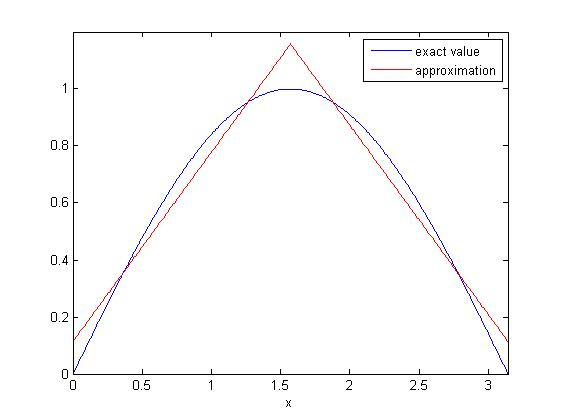
\includegraphics[width=10cm]{ex10.jpg}    % The printed column width is 8.4 cm.
\caption{Finite element approximation for $f=sin(x)$ using 2 P1 elements}
\end{center}
\end{figure}
\end{document}

